\documentclass[aps,prb,groupedaddress,nofootinbib,floatfix]{revtex4}
\usepackage{graphicx}
\usepackage{graphics}
\usepackage{epsfig}
\usepackage{url}
\usepackage[utf8]{inputenc}
\usepackage[T1]{fontenc}
\usepackage{textcomp}
\usepackage{amsmath, amssymb}
\usepackage[at]{easylist}
\usepackage{soul}
\usepackage{listings}
\usepackage{color}
\usepackage{subfig}
\usepackage{float}
\usepackage{caption}
\newfloat{map}{tbph}{lom}
\restylefloat*{map}
\floatname{map}{Map}
\captionsetup[map]{position=top}
\newcommand{\listofmaps}{\listof{map}{List of Maps}}



\definecolor{blue-violet}{rgb}{0.54, 0.17, 0.89}
\definecolor{bondiblue}{rgb}{0.0,0.58,0.71}
\definecolor{bronze}{rgb}{0.8,0.5,0.2}
\definecolor{applegreen}{rgb}{0.55,0.71,0.0}
\definecolor{arylideyellow}{rgb}{0.91,0.84,0.42}
\definecolor{grey}{rgb}{0.52,0.52,0.51}

\lstset{
	language=Python,
	aboveskip=3mm,
	belowskip=3mm,
	basicstyle={\small\ttfamily},
	numberstyle=\color{arylideyellow},
	keywordstyle=\color{bondiblue},
	commentstyle=\color{bronze},
	stringstyle=\color{applegreen},
	breaklines=true,
	showstringspaces=false,
	breakatwhitespace=true,
	tabsize=3
}
	



\pdfsuppresswarningpagegroup=1

\begin{document}
\author{Preston Seligman}
\title{Interpolation}
\date{February 21, 2025}
\maketitle
\section*{Overview} 
In this assignment, various Lagrange interpolation methods were examined and compared. These include Global interpolation, Linear interpolation, and Cubic interpolation. Interpolation methods were performed on scattering data to determine cross-sectional width, as well as over a pre-specified function.
\subsection*{Theoretical Framework} 
For N points of data of the form $(x_{i},y_{i})$, Lagrange interpolation will determine some polynomial function of degree $N-1$ such that the polynomial function will pass through each defined data point. Here, the polynomial function $f(x)$ should be a close approximation of the true function for the data/system. 
The general form of the Lagrange interpolation function $f(x)$ can be defined as
\begin{gather*}
\lambda_{i}(x)=\prod_{j=1}^{N} \left( \frac{x-x_{j}}{x_{i}-x_{j}} \right) , j \neq i\\
f(x)=\sum_{i}^{N-1} y_{i} \lambda_{i}(x)
\end{gather*}
For Global interpolation, this polynomial is calculated for all N data points, for Linear interpolation N=2, and for Cubic interpolation N=4. The error of interpolation is generally $f^{N}(\delta x)^{N}$. However, the error can vary between different interpolation methods, meaning that for different functions it may be advantageous to use one method over another.
\paragraph{Choosing Interpolation Method}
Global is beneficial as it interpolates over all data points and generates a continuous, smooth function. However, there can be issues when utilizing global interpolation, most notably of unnatural oscillations such as Runge's phenomena. Linear interpolation is easy to perform and does not have any unphysical oscillations, however it's derivative is discontinuous, and it may produce greater error if the true function is not linear. Cubic interpolation provides a happy medium; it has fewer oscillations and is reasonably smooth, however still has discontinuous derivatives at each junction. However, it can provide a better approximation than linear in cases where the true function is not linear.  
\subsection*{Code} 
\begin{lstlisting}
import matplotlib.pyplot as plt
import numpy as np

def legendrepol (x,beg,finish):          # poly interpolation at x 
    y = 0.                               # using input points from beg to finish
    for  i in range(beg,finish+1): 
       lambd = 1.0;
       for j in range(beg,finish+1):
           if i != j:                       #Lagrange polynom formed here
              lambd = lambd * ((x - xin[j])/(xin[i] - xin[j]))
       y += yin[i] * lambd
    return y

NMAX = 100  # max number of input points

xin = np.zeros(NMAX)  # each is array of length NMAX, all elements set to zero
yin = np.zeros(NMAX)

# inputfile = open("lagrange.dat","r")  # read in the input x,y values
# r = inputfile.readlines()  # read the whole file into list (one item per line)
# inputfile.close()
        # input has the form: x0 y0
        #                     x1 y1
        #                     ...
m = 0
for i in np.linspace(-1,1, num=21):
    xin[m] = i
    yin[m] = 1.0/(1.0 + (25*i**2))
    print(xin[m],yin[m])
    m += 1

    

# m = 0
# for line in r:
#     #print(line)
#     s = line.split() # split line and split into list of items(assume items separated by spaces)
#     xin[m] = s[0] # first number in each line is the x value
#     yin[m] = s[1]
#     print(xin[m],yin[m])
#     m+=1         # m is total number of input data points
#                  # will be stored in xin[0]..xin[m-1],yin[0].yin[m-1]

xvalues=range(0,201,1)  # At least 200 Steps needed to fully interpolate using our function. More will add fidelity
yval_glo = []
yval_lin = []
yval_cub = []

for x in xvalues:
    for i in range(0, m-1):
        if xin[i] <= x and x <= xin[i+1]:
            firstpoint=i
    cubepoint = firstpoint
    if cubepoint > m-4:
         cubepoint = m-4        #Need highest cubpoint to be cubepoint+3=8, so m-4=5 for this range
    yval_lin.append(legendrepol(x,firstpoint,firstpoint+1))
    yval_glo.append(legendrepol(x,0,m-1))
    yval_cub.append(legendrepol(x,cubepoint,cubepoint+3))




# for x in xvalues:         # now interpolate      
#     yvalues.append(legendrepol(x,firstpoint,firstpoint+numpoints-1))
    
plt.plot(xin[0:m],yin[0:m],"o",label="Scattering Points")
plt.plot(xvalues,yval_glo,color="orange", linewidth=1, linestyle="dashed", label="Global Interpolation")
plt.plot(xvalues,yval_lin, color="green", linewidth=2, linestyle="solid", label="Linear Interpolation")
plt.plot(xvalues,yval_cub, color="purple", linewidth=2, linestyle="dashed", label="Cubic Interpolation")
plt.legend(loc="upper right")
plt.xlabel("Energy (MeV)")
plt.ylabel("Cross Sectional Area")
plt.title("Lagrange Interpolation")
plt.axis([-1.00, 1.00, -0.2, 1.1])
plt.show()
\end{lstlisting}
\section*{Problems} 
\subsection*{Problem 1} 
First, a global interpolation of the data was performed, where interpolation was extrapolated up to 220MeV. The plot for this interpolation can be seen in Figure \ref{fig:Plot1}.
\begin{figure}[h]
	\includegraphics[width=8 cm]{Plot1.png}
	\caption{Global Interpolation Extrapolated to 220MeV}
	\label{fig:Plot1}
\end{figure}
\subsection*{Problem 2} 
Interpolation was repeated for $0\le x\le 200$ using Linear interpolation. The code for linear interpolation is
\begin{lstlisting}
for x in xvalues:
    for i in range(0, m-1):
        if xin[i] <= x and x <= xin[i+1]:
            firstpoint=i
yval_lin.append(legendrepol(x,firstpoint,firstpoint+1))
\end{lstlisting}
Here, the number of points being interpolated over is $N=2$ giving a linear function between all data points. The plot of this interpolation is given in Figure \ref{fig:Plot2}.
\begin{figure}[h]
	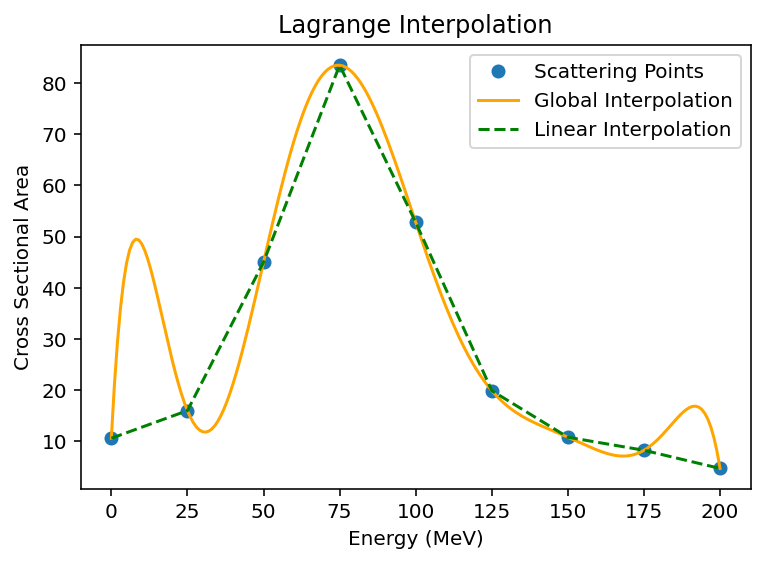
\includegraphics[width=8cm]{Plot2.png}
	\caption{Linear Interpolation}
	\label{fig:Plot2}
\end{figure}
The oscillations present in the global interpolation are no longer present for the linear interpolation. This is especially apparent near the minimum and maximum values for x.
\subsection*{Problem 3}
Cubic interpolation was performed over the same range. The code for the cubic interpolation is
\begin{lstlisting}
for x in xvalues:
    for i in range(0, m-1):
        if xin[i] <= x and x <= xin[i+1]:
            firstpoint=i
    cubepoint = firstpoint
    if cubepoint > m-4:
         cubepoint = m-4        #Need highest cubpoint to be cubepoint+3=8, so m-4=5 for this range
    yval_lin.append(legendrepol(x,firstpoint,firstpoint+1))
    yval_glo.append(legendrepol(x,0,m-1))
    yval_cub.append(legendrepol(x,cubepoint,cubepoint+3))
\end{lstlisting}
For the extreme values, the firstpoint has to be set such that $N+3$ is within the range $N$. That is to say, the cubepoint cannot be greater than $N-4$ as this will mean cubic interpolation is being performed on data outside the range. This check is performed in the function above.
The result of cubic interpolation can be seen in Figure \ref{fig:Plot3}.
\begin{figure}[h]
	\includegraphics[width=8cm]{Plot3.png}
	\caption{Cubic Interpolation}
	\label{fig:Plot3}
\end{figure}
\subsection*{Problem 4} 
These three methods of interpolation were repeated for the function $\frac{1}{1+25x^{2}}$ over the range $[-1,1]$ with 21 equally spaced intervals. The code for this function is:
\begin{lstlisting}
m = 0
for i in np.linspace(-1,1, num=21):
    xin[m] = i
    yin[m] = 1.0/(1.0 + (25*i**2))
    print(xin[m],yin[m])
    m += 1

xvalues=np.linspace(-1,1,21)

plt.plot(xvalues, yval_glo-1/(1+25*xvalues**2), linewidth=1.5, label="Gloabl Interpolation Error", color="red")
plt.plot(xvalues, yval_lin-1/(1+25*xvalues**2), linewidth=1.5, label="Linear Interpolation Error", color="green")
plt.plot(xvalues, yval_cub-1/(1+25*xvalues**2), linewidth=1.5, label="Cubic Interpolation Error", color="blue")
\end{lstlisting}
Results can be seen in Figure \ref{fig:fig1}. Error in the functions can be seen in Figure \ref{fig:fig2}.
\begin{figure}
	\centering
	\subfloat[Full Range]{\includegraphics[width=7 cm]{Plot4.png}}
	\qquad
	\subfloat[Zoomed in to Show Linear and Cubic]{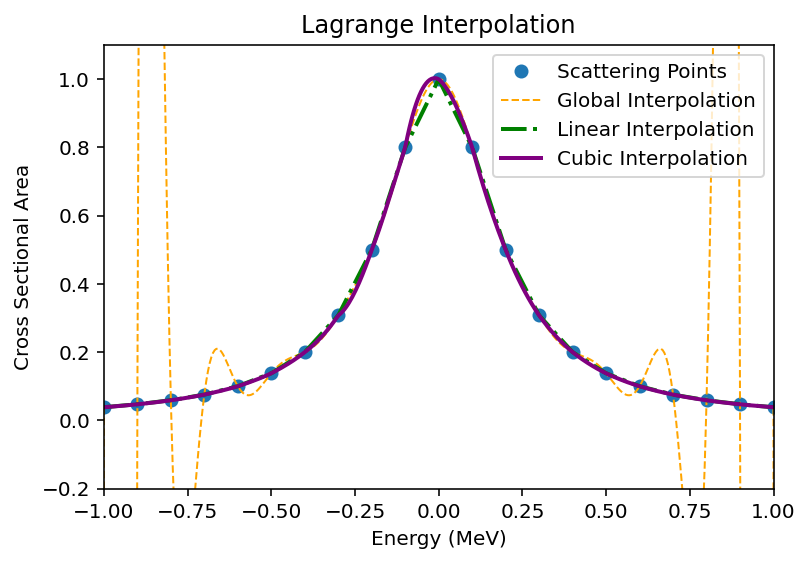
\includegraphics[width=7 cm]{Plot5.png}}
	\caption{Results for function $\frac{1}{1+25x^{2}}$}
	\label{fig:fig1}
\end{figure}
\begin{figure}
	\centering
	\subfloat[Full Range]{\includegraphics[width=7 cm]{Plot7.png}}
	\qquad
	\subfloat[Zoomed in to Show Linear and Cubic]{\includegraphics[width=7 cm]{Plot8.png}}
	\caption{Results for function $\frac{1}{1+25x^{2}}$}
	\label{fig:fig2}
\end{figure}

As can be seen, global interpolation has a large amount of oscillations. By examining the error of the functions, it can be seen that global interpolation has the lowest error near the center, however the error increases drastically as x moves further away from 0. Cubic interpolation has the lowest overall error and best approximates the data.
\end{document}
